
% !TeX program = pdflatex
\documentclass[11pt,a4paper]{article}
\usepackage[utf8]{inputenc}
\usepackage[T1]{fontenc}
\usepackage[english, turkish]{babel}
\usepackage{geometry}
\geometry{margin=2.5cm}
\usepackage{graphicx}
\usepackage{booktabs}
\usepackage{siunitx}
\usepackage{hyperref}
\usepackage{caption}
\usepackage{subcaption}
\usepackage{amsmath}

\title{KarabukWildfire2025: Sentinel-2 ile NDVI/NBR Tabanlı Yangın Etki Analizi}
\author{Yusuf Talha ARABACI\\Karabük Üniversitesi\\Yüksek Lisans, Yazılım Mühendisliği Öğrencisi}
\date{Tarih: \today}

\begin{document}
\maketitle
\thispagestyle{empty}

\clearpage
\tableofcontents
\clearpage

% Turkish abstract (Özet)
\selectlanguage{turkish}
\renewcommand{\abstractname}{Özet}
\begin{abstract}
Bu çalışma, 2025 Karabük orman yangınının etkilerini Sentinel-2 L2A verileri kullanılarak
NDVI ve NBR indeksleri üzerinden incelemektedir. Yangın öncesi ve sonrası dönemler için
bulut maskeleme ve median kompozit uygulandıktan sonra NDVI/NBR bantları hesaplanmış,
fark indeksleri (dNDVI, dNBR) türetilmiş ve dNBR eşiklerine dayalı bir şiddet sınıflandırması
gerçekleştirilmiştir. Sonuçlar, doğal renk (RGB) ve tematik haritalar ile özet istatistikler
eşliğinde sunulmaktadır. Yaklaşım, uzaktan algılama temelli hızlı durum değerlendirmesi ve
afet sonrası planlama süreçlerine katkı sağlamayı amaçlamaktadır.
\end{abstract}

\clearpage

\section{Giriş}
2025 Karabük orman yangınlarının ekosistem, toprak ve yerleşimler üzerindeki etkilerinin
nicel ve mekânsal olarak ortaya konması; yangın sonrası rehabilitasyon, yeniden
ormanlaştırma ve risk azaltma planlamaları açısından kritik öneme sahiptir. Uzaktan
algılama, yüksek zamansal ve mekânsal çözünürlükte tekrarlanan gözlemleri mümkün kılarak
yangın öncesi/sonrası karşılaştırmalı analizlerin sistematik biçimde yürütülmesine imkân
tanır. Bu çalışma, Sentinel-2 L2A verileriyle \emph{Normalized Difference Vegetation Index}
(NDVI) ve \emph{Normalized Burn Ratio} (NBR) indekslerine dayanan bir yaklaşım
sunmaktadır; fark indeksleri (dNDVI, dNBR) ve eşik tabanlı şiddet sınıflandırması ile
etki alanı haritaları üretilmektedir.

\section{Çalışma Alanı (AOI)}
Çalışma alanı, Karabük ili Ovacık--Eskipazar çevresi ve doğuda Çankırı sınırına
komşu bir bölgeyi kapsamaktadır. AOI, depo kökünde yer alan \texttt{src/aoi.geojson}
dosyasında çokgen (Polygon) olarak tanımlanmıştır. Bu AOI, yangınla doğrudan ilişkili
alanları kapsayacak şekilde iteratif olarak daraltılmış ve sonuç analizlerinde esas
alınmıştır.

\section{Proje Amacı}
Bu çalışmanın amacı, yangın öncesi ve sonrası dönemler için NDVI ve NBR indekslerini
hesaplayarak, fark (dNDVI, dNBR) analizi ve basit bir şiddet sınıflandırması ile
yangından etkilenen alanları ortaya koymaktır.

\section{Veri Kaynakları}

\par
\textbf{Uydu verisi:} Sentinel-2 Level-2A atmosferik olarak düzeltilmiş yansıtım
ürünleri; mekânsal çözünürlük 10--20 m. Bu çalışmada NDVI için B8 (NIR) ve B4 (RED),
NBR için B8 (NIR) ve B12 (SWIR2) bantları kullanılmıştır.
\par
\textbf{Platform:} Google Earth Engine (GEE) Python API, geniş hacimli veri erişimi ve
dağıtık hesaplama altyapısı ile iş akışının ölçeklenebilir yürütümünü sağlar.
\par
\textbf{Bulut maskesi:} Sentinel-2 QA60 kalite bandındaki 10. (bulut) ve 11. (sirrus)
bitleri sıfır olan pikseller geçerli kabul edilmiştir.
\par
\textbf{Kompozit:} Her dönem için median kompozit, tekil bulut kalıntılarını ve uç
değerleri azaltmak üzere tercih edilmiştir.

\section{Görüntü İşleme Teknikleri}
\subsection*{NDVI}
\begin{equation}
\mathrm{NDVI} = \frac{\mathrm{NIR}-\mathrm{RED}}{\mathrm{NIR}+\mathrm{RED}}\,, \quad
\text{(S2: NIR=B8, RED=B4)}
\end{equation}
\subsection*{NBR}
\begin{equation}
\mathrm{NBR} = \frac{\mathrm{NIR}-\mathrm{SWIR2}}{\mathrm{NIR}+\mathrm{SWIR2}}\,, \quad
\text{(S2: NIR=B8, SWIR2=B12)}
\end{equation}
\subsection*{Fark İndeksleri}
\begin{align}
\mathrm{dNDVI} &= \mathrm{NDVI}_{\text{sonra}} - \mathrm{NDVI}_{\text{önce}}\\
\mathrm{dNBR}  &= \mathrm{NBR}_{\text{önce}} - \mathrm{NBR}_{\text{sonra}}
\end{align}
Pozitif dNBR değerleri yanıklığın arttığı bölgeleri işaret ederken, negatif dNDVI
değerleriyle birlikte yorumlandığında vejetasyon kaybına ilişkin güçlü kanıt sağlar.

\subsection*{NDVI ve NBR: Tanım, Yorum ve Sınırlılıklar}
\textbf{NDVI} (Normalized Difference Vegetation Index), \([-1,1]\) aralığında
boyutsuz bir ölçüttür vejetasyonun göreli canlılık ve yoğunluğunu yansıtır.
Genellikle \(0.5{-}0.9\) aralığı sağlıklı/yoğun bitki örtüsünü, orta değerler karışık
örtü/çıplak toprak etkisini, düşük/negatif değerler ise su/kar/çıplak kaya ve yapay
yüzeyleri işaret eder. \textbf{NBR} (Normalized Burn Ratio) ise yangın sonrası
gözlenen spektral değişimlere (NIR azalışı, SWIR2 artışı) duyarlıdır; yangın öncesi
yüksek, sonrası düşük olması beklenir. \textbf{dNBR} tanımı gereği pozitif ve büyük
değerler daha yüksek yanıklık şiddetine karşılık gelir. Her iki indeks de atmosferik
koşullar, toprak arka planı, aydınlatma geometrisi ve sensör/saha farklılıklarından
etkilenebilir; bu nedenle fark indeksleri (önce/sonra) ve maskeleme/kompozit adımları
yorumlanabilirliği güçlendirir.

\subsection*{Neden NDVI ve NBR?}
Bu çalışma, \textbf{NDVI} ve \textbf{NBR} indekslerini tercih etmiştir çünkü:
\begin{itemize}
  \item \textbf{Yaygın ve kanıtlı kullanım:} Yangın etkisi ve bitki örtüsü değişimi çalışmalarında literatürde en yaygın iki fark indikatörüdür (dNDVI, dNBR).
  \item \textbf{Duyarlılık:} NDVI klorofil/vejetasyon canlılığına duyarlıyken, NBR yanıklık ve yanmış artıkların (NIR düşüşü, SWIR2 artışı) etkisini yakalar.
  \item \textbf{Uyarlanabilirlik:} dNBR için eşik temelli şiddet sınıflandırma basit ve yorumlanabilirdir; saha verisiyle kolayca kalibre edilebilir.
  \item \textbf{Erişilebilirlik:} Gerekli bantlar (B8, B4, B12) Sentinel-2 L2A'da 10--20 m çözünürlükte düzenli olarak mevcuttur.
\end{itemize}
Alternatif olarak \emph{EVI}, \emph{SAVI}, \emph{RdNBR} gibi indeksler de değerlendirilebilir; ancak bu çalışmada doğruluğu/yorumlanabilirliği yüksek, uygulaması pratik iki temel indeks üzerinden ilerlemek hedeflenmiştir.

\section{Yöntem}
Yaklaşımımızın iş akışı şu adımlardan oluşmaktadır: (i) tarih aralığı seçimi ve veri
erişimi, (ii) QA60 tabanlı bulut/sirrus maskesi, (iii) median kompozit üretimi,
(iv) NDVI/NBR indekslerinin hesaplanması, (v) dNDVI/dNBR farklarının elde edilmesi,
ve (vi) dNBR eşiklerine dayalı şiddet sınıflandırması. Sınıflandırma için eşikler
temsilidir ve AOI/saha koşullarına göre güncellenebilir.

\subsection*{Analiz Hattı (pipeline.py)}
Çalışmadaki analiz süreci \texttt{src/pipeline.py} içinde tanımlı \texttt{run\_pipeline} işleviyle otomatikleştirilmiştir. Başlıca adımlar ve üretilen çıktılar şöyledir:
\begin{itemize}
  \item \textbf{Başlatma ve AOI:} \texttt{ee\_init} ile Google Earth Engine başlatılır; \texttt{get\_aoi} ile AOI GeoJSON'dan (yoksa varsayılan bbox) yüklenir.
  \item \textbf{Kompozitler:} \texttt{prepare\_composite} ile öncesi ve sonrası dönem için QA60 maskeleme uygulanmış Sentinel-2 median kompozitleri üretilir.
  \item \textbf{İndeksler:} \texttt{with\_indices} NDVI (B8,B4) ve NBR (B8,B12) bantlarını her iki kompozite ekler.
  \item \textbf{Farklar:} \texttt{compute\_diffs} ile $\mathrm{dNDVI} = \mathrm{post.NDVI} - \mathrm{pre.NDVI}$ ve $\mathrm{dNBR} = \mathrm{pre.NBR} - \mathrm{post.NBR}$ görüntüleri hesaplanır.
  \item \textbf{Şiddet:} \texttt{classify\_dnbr} dNBR için 0–4 arası şiddet sınıflarını (eşik temelli) üretir.
  \item \textbf{Haritalar:} \texttt{save\_folium} ile şu HTML haritaları kaydedilir: \texttt{pre\_RGB.html}, \texttt{post\_RGB.html}, \texttt{pre\_NDVI.html}, \texttt{post\_NDVI.html}, \texttt{pre\_NBR.html}, \texttt{post\_NBR.html}, \texttt{dNDVI.html}, \texttt{dNBR.html}, \texttt{severity.html}.
  \item \textbf{Özet istatistik:} \texttt{reduce\_mean} ile AOI üzerinde öncesi/sonrası NDVI ortalamaları ve dNDVI/dNBR ortalamaları hesaplanır; \texttt{write\_summary\_csv} ile \texttt{results/summary\_stats.csv} dosyasına yazılır.
\end{itemize}

Bu çalışmada pipeline, öncesi için \texttt{2025-07-10--2025-07-25}, sonrası için \texttt{2025-07-26--2025-08-10} tarih aralıklarıyla çalıştırılmıştır. Üretilen \texttt{results/summary\_stats.csv} dosyasındaki değerler rapordaki özet istatistik tablosu ve yorumlarda kullanılmıştır.

\noindent \emph{Komut satırından örnek kullanım:}

\noindent\texttt{python -m src.cli --pre-start 2025-07-10 --pre-end 2025-07-25 --post-start 2025-07-26 --post-end 2025-08-10 --aoi data/aoi.geojson --out results}

\subsection*{Parametre Seçimleri ve Uygulama Ayrıntıları}
\begin{itemize}
  \item \textbf{Bulut eşiği:} Koleksiyon seçiminde \texttt{CLOUDY\_PIXEL\_PERCENTAGE} $<20$
  filtresi uygulanmış, ardından QA60 bitleriyle piksel düzeyinde bulut/sirrus maskesi
  kullanılmıştır.
  \item \textbf{Kompozit stratejisi:} Median kompozit, uç değerleri bastırması ve
  yapay parazitleri azaltması nedeniyle tercih edilmiştir.
  \item \textbf{Eşikler:} dNBR sınıfları literatürde önerilen aralıklardan uyarlanmış
  olup yerel AOI’ye/saha gözlemlerine göre kalibre edilebilir.
\end{itemize}

\subsection*{Yanıklık Şiddeti Sınıflandırması}
\begin{table}[h]
  \centering
  \begin{tabular}{@{}lll@{}}\toprule
  Sınıf & Kod & dNBR Eşiği \\\midrule
  Yanıksız/Düşük & 0 & $\leq 0.10$ \\
  Düşük & 1 & $(0.10,\,0.27]$ \\
  Orta--Düşük & 2 & $(0.27,\,0.44]$ \\
  Orta--Yüksek & 3 & $(0.44,\,0.66]$ \\
  Yüksek & 4 & $> 0.66$ \\\bottomrule
  \end{tabular}
  \caption{dNBR eşikleri ile önerilen şiddet sınıfları (örnek).}
\end{table}

Bu bölümde sunulan özet, yangın öncesi ve sonrası bitki örtüsü durumunu (NDVI) ve yangın etkisini (dNBR) nicel olarak ifade eder. NDVI 0 ile 1 arasında değer alır; daha yüksek değerler daha yoğun ve sağlıklı bitki örtüsünü gösterir. dNDVI iki tarih arasındaki NDVI farkıdır; negatif değerler yeşil örtüde azalmayı ifade eder. dNBR ise yanma şiddetine duyarlı bir fark ölçütüdür; yaklaşık 0.10--0.27 aralığı düşük, 0.27--0.44 aralığı orta, 0.44 ve üzeri daha yüksek şiddet seviyelerine karşılık gelir. Tablodaki ortalamalar, AOI genelinde yangın sonrası NDVI’da yaklaşık 0.06 birimlik düşüş (yaklaşık 0.54'ten 0.47'ye; \(dNDVI<0\)) ve \(dNBR \approx 0.07\) ile çoğunlukla çok düşük/düşük şiddet sinyaline işaret etmektedir. Ancak bu değerler mekânsal farklılıkları düzler; yer yer daha yüksek şiddetli cepler bulunabilir. Bu nedenle yorum, şiddet haritaları ve sınıf dağılımı ile birlikte değerlendirilmelidir.

Sınıf piksel sayıları üzerinden alan hesaplanabilir. Örneğin, piksel alanı \SI{100}{m\textsuperscript{2}}
(10 m çözünürlükte) ise, sınıf alanı $A_k = n_k \times 100\,\mathrm{m^2}$ olup
hektar cinsinden $A_k/10^4$ ile verilir.

\section{Sonuçlar}
\subsection*{Harita Yer Tutucuları}
\begin{figure}[h]
  \centering
  \begin{subfigure}[b]{0.48\textwidth}
    \centering
    \resizebox{\linewidth}{!}{\includegraphics{../results/pre_RGB.png}}
    \caption{Öncesi RGB (B4,B3,B2)}
  \end{subfigure}\hfill
  \begin{subfigure}[b]{0.48\textwidth}
    \centering
    \resizebox{\linewidth}{!}{\includegraphics{../results/post_RGB.png}}
    \caption{Sonrası RGB (B4,B3,B2)}
  \end{subfigure}
  \caption{Doğal renk (RGB) karşılaştırması.}
\end{figure}

\begin{figure}[h]
  \centering
  \begin{subfigure}[b]{0.48\textwidth}
    \centering
    \resizebox{\linewidth}{!}{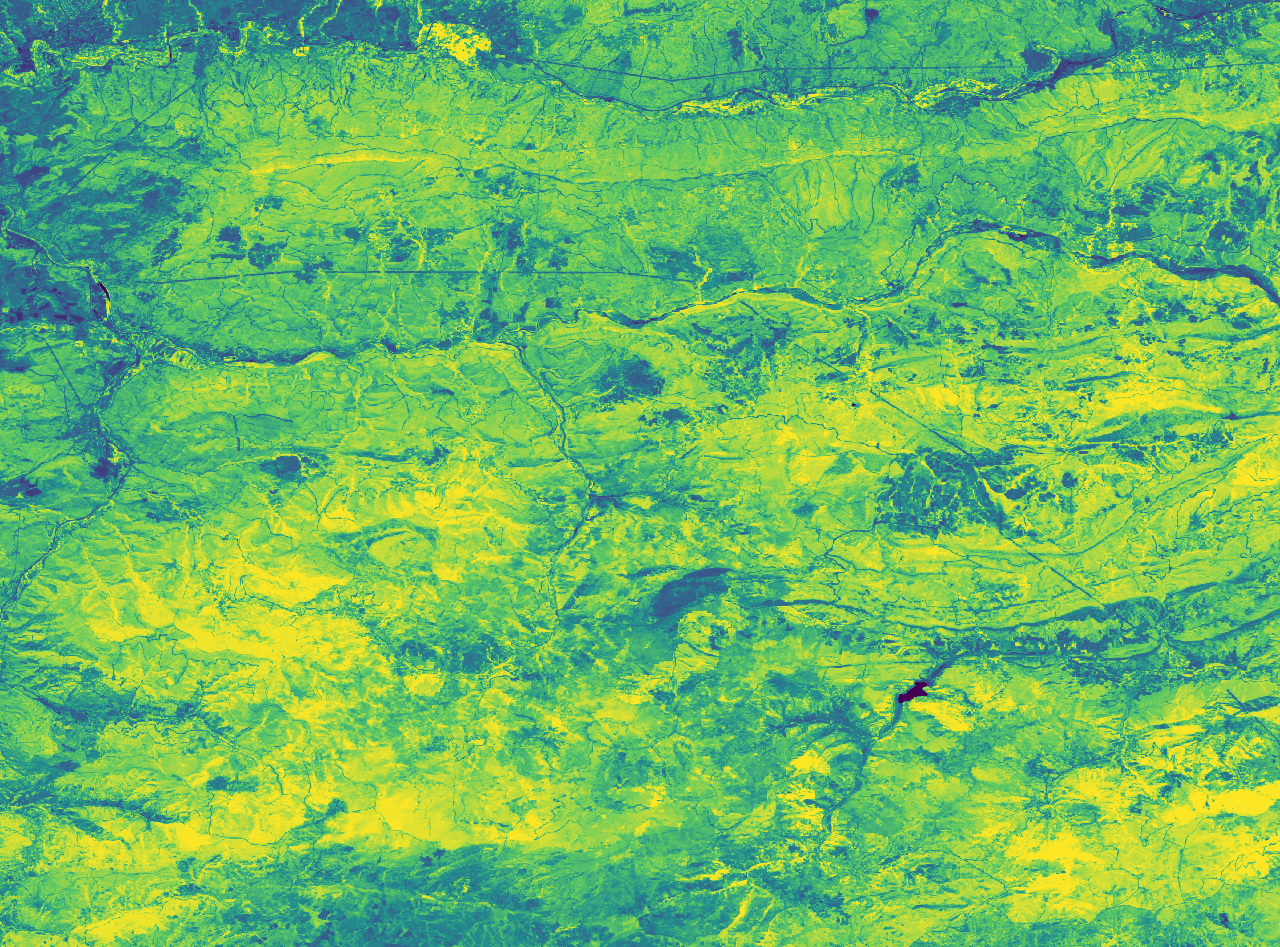
\includegraphics{../results/pre_NDVI.png}}
    \caption{Öncesi NDVI}
  \end{subfigure}\hfill
  \begin{subfigure}[b]{0.48\textwidth}
    \centering
    \resizebox{\linewidth}{!}{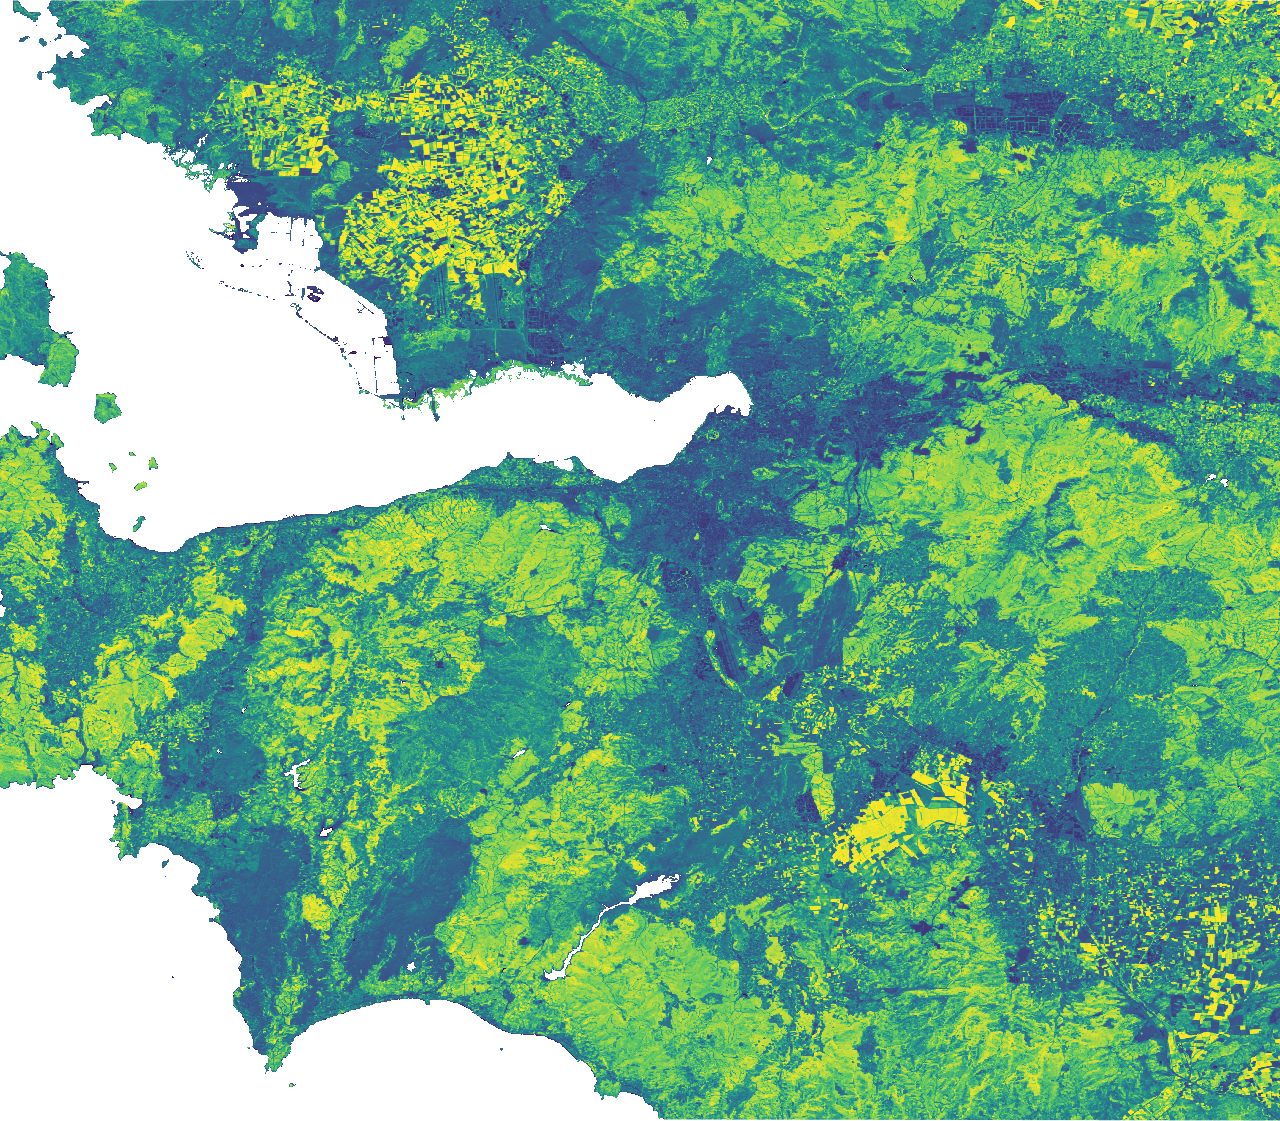
\includegraphics{../results/post_NDVI.png}}
    \caption{Sonrası NDVI}
  \end{subfigure}
  \caption{NDVI karşılaştırması.}
\end{figure}

\begin{figure}[h]
  \centering
  \begin{subfigure}[b]{0.48\textwidth}
    \centering
    \resizebox{\linewidth}{!}{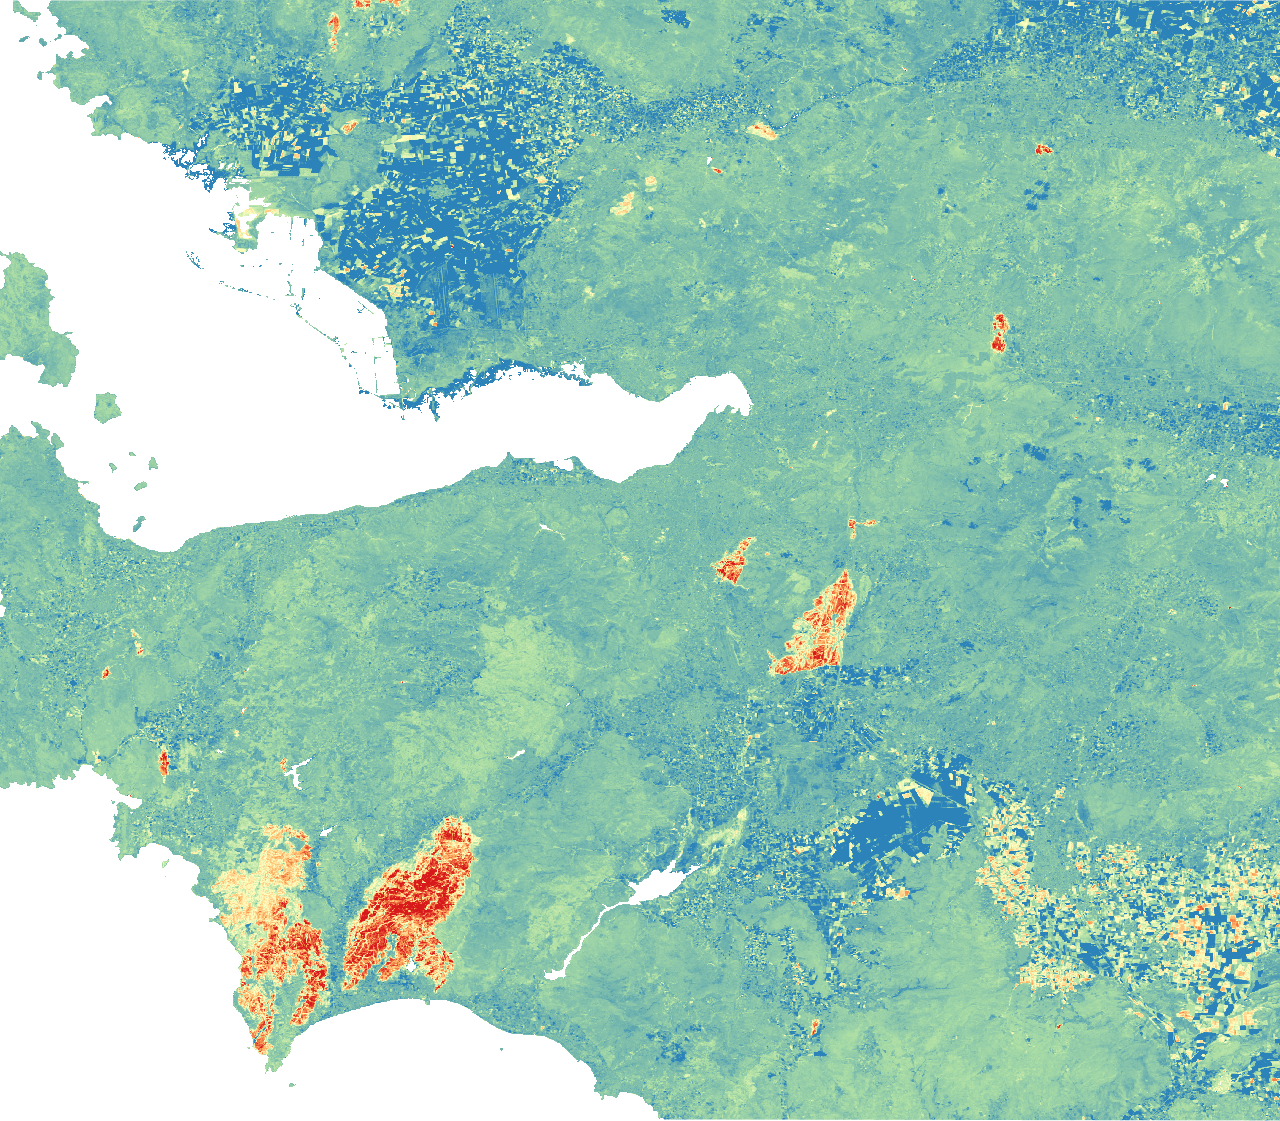
\includegraphics{../results/dNBR.png}}
    \caption{dNBR}
  \end{subfigure}\hfill
  \begin{subfigure}[b]{0.48\textwidth}
    \centering
    \resizebox{\linewidth}{!}{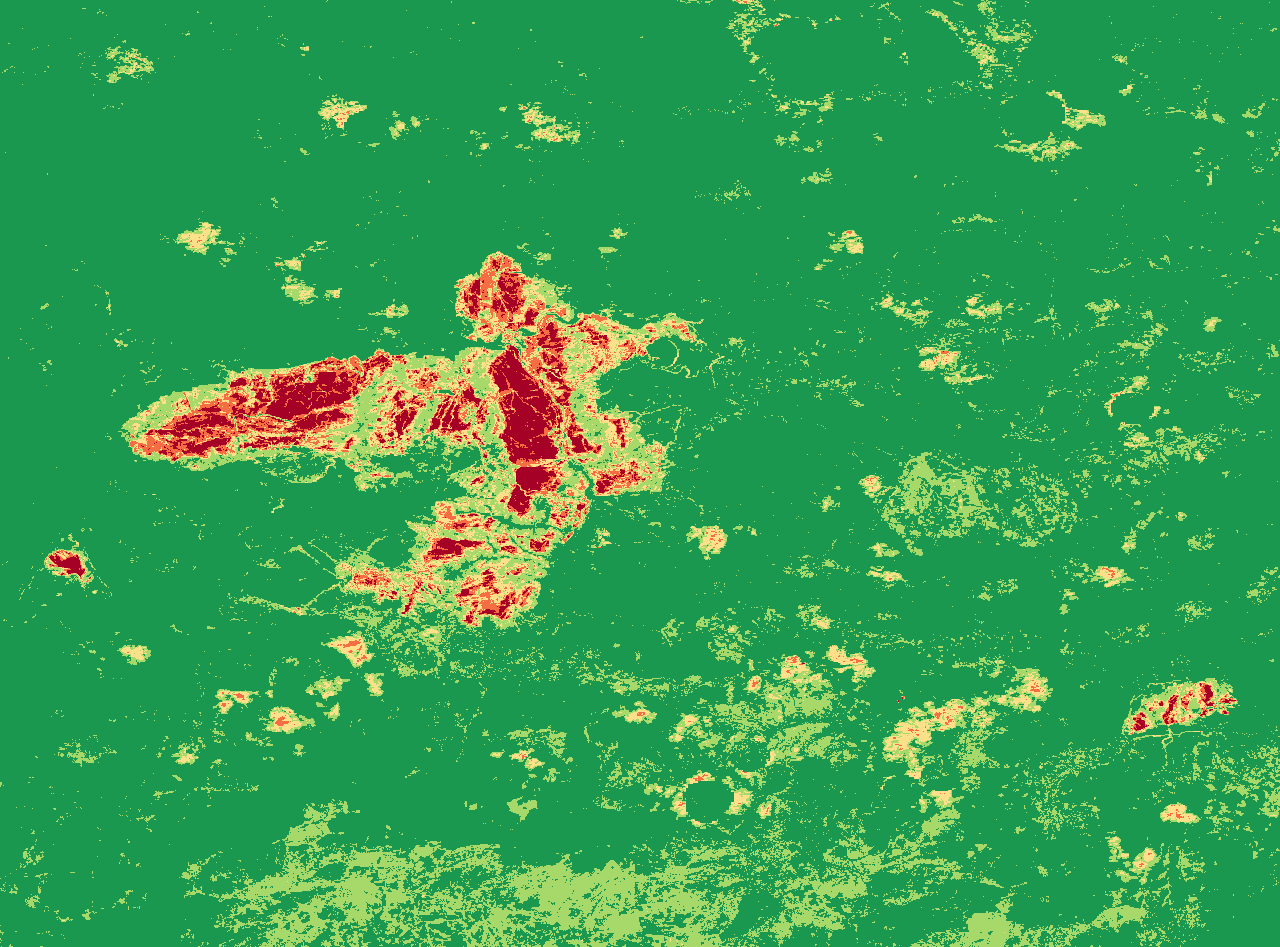
\includegraphics{../results/severity.png}}
    \caption{dNBR Şiddeti (0--4)}
  \end{subfigure}
  \caption{Fark analizi ve şiddet sınıfları.}
\end{figure}

\subsection*{Özet İstatistikler}
\begin{table}[h]
  \centering
  \begin{tabular}{@{}ll@{}}\toprule
  Metrik & Değer \\\midrule
  Öncesi Ortalama NDVI & 0.54 \\
  Sonrası Ortalama NDVI & 0.47 \\
  Ortalama dNDVI & $-0.06$ \\
  Ortalama dNBR & 0.07 \\\bottomrule
  \end{tabular}
  \caption{AOI genelinde özet istatistikler (örnek yer tutucu). Gerçek değerlere \texttt{../results/summary\_stats.csv} dosyasından erişilebilir.}
\end{table}

Bu bölümde sunulan özet, yangın öncesi ve sonrası bitki örtüsü durumunu (NDVI) ve yangın etkisini (dNBR) nicel olarak ifade eder. NDVI 0 ile 1 arasında değer alır; daha yüksek değerler daha yoğun ve sağlıklı bitki örtüsünü gösterir. dNDVI iki tarih arasındaki NDVI farkıdır; negatif değerler yeşil örtüde azalmayı ifade eder. dNBR ise yanma şiddetine duyarlı bir fark ölçütüdür; yaklaşık 0.10--0.27 aralığı düşük, 0.27--0.44 aralığı orta, 0.44 ve üzeri daha yüksek şiddet seviyelerine karşılık gelir. Tablodaki ortalamalar, AOI genelinde yangın sonrası NDVI’da yaklaşık 0.06 birimlik düşüş (yaklaşık 0.54'ten 0.47'ye; \(dNDVI<0\)) ve \(dNBR \approx 0.07\) ile çoğunlukla çok düşük/düşük şiddet sinyaline işaret etmektedir. Ancak bu değerler mekânsal farklılıkları düzler; yer yer daha yüksek şiddetli cepler bulunabilir. Bu nedenle yorum, şiddet haritaları ve sınıf dağılımı ile birlikte değerlendirilmelidir.

Etkilenen alan büyüklükleri, sınıf piksel sayıları ve/veya eşiklerin literatürle
karşılaştırılması ek bir tablo olarak verilebilir.

\section{Sınırlılıklar ve Belirsizlikler}
Bulut ve duman kalıntıları, geometrik/atmosferik kalıntı hataları ve sınıflandırma
eşiklerinin genellenebilirliği sonuçları etkileyebilir. dNBR eşikleri AOI'ye ve saha
gözlemlerine göre kalibre edilmelidir. Kompozit stratejisinin (median) seçimi mekânsal
özgüllük ve bulutluluk koşullarına bağlıdır.

\section{Tartışma ve Gelecek Çalışmalar}
Yöntem, GEE altyapısıyla hızlı ve tekrarlanabilir analiz sağlar. Gelecekte RdNBR gibi
normalize edilmiş fark metriklerinin denenmesi; arazi örtüsü/sınıf bilgisi ile
birleştirilmiş analizler ve saha verisiyle karşılaştırmalı doğrulama, karar destek
perspektifinden yöntemin değerini artıracaktır. Ayrıca farklı sensörlerle (Landsat,\,Sentinel-1)
çoklu-kaynak yaklaşımı geliştirilerek zamansal kapsam ve sağlamlık genişletilebilir.

\section{Görselleştirme}
Harita görselleri, \texttt{analysis.ipynb} defterinden otomatik üretilen HTML ve PNG
çıktıları üzerinden alınmıştır. Renk paletleri ve gösterim aralıkları \texttt{src/visualize.py}
dosyasında \texttt{vis\_params()} fonksiyonunda tanımlıdır.

\section{Sonuç ve Tartışma}
Sunulan yöntem, GEE üzerinde hızlı ve tekrarlanabilir bir akışla yangın etkilerini
haritalandırmaktadır. Eşiklerin saha verileri ile kalibre edilmesi ve farklı
zaman aralıklarının denenmesiyle, hem doğruluk hem de yorumlanabilirlik artacaktır.
Gelecek çalışmalarda, \emph{Relative dNBR (RdNBR)} ve arazi örtüsü sınıflarıyla
birleşik değerlendirmeler önerilir.

\end{document}
% !TeX program = pdflatex
\documentclass[11pt,a4paper]{article}
\usepackage[utf8]{inputenc}
\usepackage[T1]{fontenc}
\usepackage[turkish]{babel}
\usepackage{geometry}
\geometry{margin=2.5cm}
\usepackage{graphicx}
\usepackage{subcaption}
\usepackage{booktabs}
\usepackage{siunitx}
\usepackage{amsmath}
\usepackage{microtype}
\usepackage{caption}
\usepackage{hyperref}
\graphicspath{{../results/}}
\captionsetup[table]{position=bottom}
\hypersetup{colorlinks=true, linkcolor=blue, urlcolor=blue, citecolor=blue}

\title{KarabukWildfire2025: Sentinel-2 ile NDVI/NBR Tabanlı Yangın Etki Analizi}
\author{Yusuf Talha ARABACI\\Karabük Üniversitesi\\Yüksek Lisans, Yazılım Mühendisliği }
\date{Tarih: \today}

\begin{document}
\maketitle
\thispagestyle{empty}
\clearpage
\tableofcontents
\clearpage

\begin{abstract}
Bu çalışma, 2025 Karabük orman yangınının etkilerini Sentinel-2 L2A verileri kullanılarak
NDVI ve NBR indeksleri üzerinden incelemektedir. Yangın öncesi ve sonrası dönemler için
bulut maskeleme ve median kompozit uygulandıktan sonra NDVI/NBR bantları hesaplanmış,
fark indeksleri (dNDVI, dNBR) türetilmiş ve dNBR eşiklerine dayalı bir şiddet sınıflandırması
gerçekleştirilmiştir. Sonuçlar, doğal renk (RGB) ve tematik haritalar ile özet istatistikler
eşliğinde sunulmaktadır. Yaklaşım, uzaktan algılama temelli hızlı durum değerlendirmesi ve
afet sonrası planlama süreçlerine katkı sağlamayı amaçlamaktadır.
\end{abstract}
\noindent\textbf{Anahtar Kelimeler:} Karabük, orman yangını, Sentinel-2, NDVI, NBR, dNBR, Google Earth Engine

\par\medskip
% English abstract (Abstract)
\selectlanguage{english}
\renewcommand{\abstractname}{Abstract}
\begin{abstract}
This study analyzes the impacts of the 2025 Karabük wildfire using Sentinel-2 L2A data. We compute NDVI and NBR for pre- and post-fire periods, derive difference indices (dNDVI, dNBR), and perform a threshold-based burn severity classification on dNBR. Cloud and cirrus masking (QA60) and median compositing are applied for each period. Results are presented with true-color (RGB) and thematic maps and area-wide summary statistics. The workflow, implemented on Google Earth Engine, aims to support rapid situational assessment and post-fire planning.
\end{abstract}
\noindent\textbf{Keywords:} Karabuk, wildfire, Sentinel-2, NDVI, NBR, dNBR, Google Earth Engine
\selectlanguage{turkish}
\clearpage

\section{Giriş}
2025 Karabük orman yangınlarının ekosistem, toprak ve yerleşimler üzerindeki etkilerinin
nicel ve mekânsal olarak ortaya konması; yangın sonrası rehabilitasyon, yeniden
ormanlaştırma ve risk azaltma planlamaları açısından kritik öneme sahiptir. Uzaktan
algılama, yüksek zamansal ve mekânsal çözünürlükte tekrarlanan gözlemleri mümkün kılarak
yangın öncesi/sonrası karşılaştırmalı analizlerin sistematik biçimde yürütülmesine imkân
tanır. Bu çalışma, Sentinel-2 L2A verileriyle \emph{Normalized Difference Vegetation Index}
(NDVI) ve \emph{Normalized Burn Ratio} (NBR) indekslerine dayanan bir yaklaşım
sunmaktadır; fark indeksleri (dNDVI, dNBR) ve eşik tabanlı şiddet sınıflandırması ile
etki alanı haritaları üretilmektedir.

\section{Çalışma Alanı (AOI)}
Çalışma alanı, Karabük ili Ovacık--Eskipazar çevresi ve doğuda Çankırı sınırına
komşu bir bölgeyi kapsamaktadır. AOI, depo kökünde yer alan \texttt{src/aoi.geojson}
dosyasında çokgen (Polygon) olarak tanımlanmıştır. Bu AOI, yangınla doğrudan ilişkili
alanları kapsayacak şekilde iteratif olarak daraltılmış ve sonuç analizlerinde esas
alınmıştır.

\section{Proje Amacı}
Bu çalışmanın amacı, yangın öncesi ve sonrası dönemler için NDVI ve NBR indekslerini
hesaplayarak, fark (dNDVI, dNBR) analizi ve basit bir şiddet sınıflandırması ile
yangından etkilenen alanları ortaya koymaktır.
\paragraph{Araştırma Soruları} (i) Yangın sonrasında AOI genelinde vejetasyon canlılığındaki
değişim (dNDVI) nedir ve mekânsal dağılımı nasıldır? (ii) dNBR temelli şiddet sınıfları
hangi bölgelerde yoğunlaşmaktadır? (iii) Hangi sınıflar alan açısından baskındır ve bu
dağılım, saha/yerel bilgiyle tutarlı mıdır?

\section{Veri Kaynakları}
\textbf{Uydu verisi:} Sentinel-2 Level-2A atmosferik olarak düzeltilmiş yansıtım
ürünleri; mekânsal çözünürlük 10--20 m. Bu çalışmada NDVI için B8 (NIR) ve B4 (RED),
NBR için B8 (NIR) ve B12 (SWIR2) bantları kullanılmıştır.\par
\textbf{Platform:} Google Earth Engine (GEE) Python API, geniş hacimli veri erişimi ve
dağıtık hesaplama altyapısı ile iş akışının ölçeklenebilir yürütümünü sağlar \cite{Drusch2012}.\par
\textbf{Bulut maskesi:} Sentinel-2 QA60 kalite bandındaki 10. (bulut) ve 11. (sirrus)
bitleri sıfır olan pikseller geçerli kabul edilmiştir.\par
\textbf{Kompozit:} Her dönem için median kompozit, tekil bulut kalıntılarını ve uç
değerleri azaltmak üzere tercih edilmiştir.

\section{Görüntü İşleme Teknikleri}
\subsection*{NDVI}
\begin{equation}
\mathrm{NDVI} = \frac{\mathrm{NIR}-\mathrm{RED}}{\mathrm{NIR}+\mathrm{RED}}\,, \quad
\text{(S2: NIR=B8, RED=B4)}
\end{equation}\, (bkz. \cite{Rouse1973})
\subsection*{NBR}
\begin{equation}
\mathrm{NBR} = \frac{\mathrm{NIR}-\mathrm{SWIR2}}{\mathrm{NIR}+\mathrm{SWIR2}}\,, \quad
\text{(S2: NIR=B8, SWIR2=B12)}
\end{equation}\, (bkz. \cite{KeyBenson2006})
\subsection*{Fark İndeksleri}
\begin{align}
\mathrm{dNDVI} &= \mathrm{NDVI}_{\text{sonra}} - \mathrm{NDVI}_{\text{önce}}\\
\mathrm{dNBR}  &= \mathrm{NBR}_{\text{önce}} - \mathrm{NBR}_{\text{sonra}}
\end{align}
Pozitif dNBR değerleri yanıklığın arttığı bölgeleri işaret ederken, negatif dNDVI
değerleriyle birlikte yorumlandığında vejetasyon kaybına ilişkin güçlü kanıt sağlar.

\subsection*{NDVI ve NBR: Tanım, Yorum ve Sınırlılıklar}
\textbf{NDVI} (Normalized Difference Vegetation Index), \([-1,1]\) aralığında
boyutsuz bir ölçüttür vejetasyonun göreli canlılık ve yoğunluğunu yansıtır.
Genellikle \(0.5{-}0.9\) aralığı sağlıklı/yoğun bitki örtüsünü, orta değerler karışık
örtü/çıplak toprak etkisini, düşük/negatif değerler ise su/kar/çıplak kaya ve yapay
yüzeyleri işaret eder. \textbf{NBR} (Normalized Burn Ratio) ise yangın sonrası
gözlenen spektral değişimlere (NIR azalışı, SWIR2 artışı) duyarlıdır; yangın öncesi
yüksek, sonrası düşük olması beklenir. \textbf{dNBR} tanımı gereği pozitif ve büyük
değerler daha yüksek yanıklık şiddetine karşılık gelir. Her iki indeks de atmosferik
koşullar, toprak arka planı, aydınlatma geometrisi ve sensör/saha farklılıklarından
etkilenebilir; bu nedenle fark indeksleri (önce/sonra) ve maskeleme/kompozit adımları
yorumlanabilirliği güçlendirir.

\subsection*{Neden NDVI ve NBR?}
Bu çalışma, \textbf{NDVI} ve \textbf{NBR} indekslerini tercih etmiştir çünkü:
\begin{itemize}
  \item \textbf{Yaygın ve kanıtlı kullanım:} Yangın etkisi ve bitki örtüsü değişimi çalışmalarında literatürde en yaygın iki fark indikatörüdür (dNDVI, dNBR).
  \item \textbf{Duyarlılık:} NDVI klorofil/vejetasyon canlılığına duyarlıyken, NBR yanıklık ve yanmış artıkların (NIR düşüşü, SWIR2 artışı) etkisini yakalar.
  \item \textbf{Uyarlanabilirlik:} dNBR için eşik temelli şiddet sınıflandırma basit ve yorumlanabilirdir; saha verisiyle kolayca kalibre edilebilir.
  \item \textbf{Erişilebilirlik:} Gerekli bantlar (B8, B4, B12) Sentinel-2 L2A'da 10--20 m çözünürlükte düzenli olarak mevcuttur.
\end{itemize}
Alternatif olarak \emph{EVI}, \emph{SAVI}, \emph{RdNBR} gibi indeksler de değerlendirilebilir; ancak bu çalışmada doğruluğu/yorumlanabilirliği yüksek, uygulaması pratik iki temel indeks üzerinden ilerlemek hedeflenmiştir.

\section{Yöntem}
Yaklaşımımızın iş akışı şu adımlardan oluşmaktadır: (i) tarih aralığı seçimi ve veri
erişimi, (ii) QA60 tabanlı bulut/sirrus maskesi, (iii) median kompozit üretimi,
(iv) NDVI/NBR indekslerinin hesaplanması, (v) dNDVI/dNBR farklarının elde edilmesi,
ve (vi) dNBR eşiklerine dayalı şiddet sınıflandırması. Sınıflandırma için eşikler
temsilidir ve AOI/saha koşullarına göre güncellenebilir.

\subsection*{Analiz Hattı (pipeline.py)}
Analiz akışı \texttt{src/pipeline.py} içindeki \texttt{run\_pipeline} ile uçtan uca yürütülmüştür. Özetle: (i) GEE başlatma ve AOI yükleme; (ii) öncesi/sonrası median kompozit ve NDVI/NBR hesaplama; (iii) dNDVI/dNBR fark katmanları ve dNBR şiddet sınıfları; (iv) Folium tabanlı haritaların ve \texttt{summary\_stats.csv} özetlerinin yazılması. Çalışmada kullanılan tarih aralıkları: \texttt{2025-07-10--2025-07-25} (öncesi) ve \texttt{2025-07-26--2025-08-10} (sonrası). Çıktılar \texttt{results/} klasörüne kaydedilir ve rapordaki tablo/figürlerde kullanılmıştır.

\subsection*{Parametre Seçimleri ve Uygulama Ayrıntıları}
\begin{itemize}
  \item \textbf{Bulut eşiği:} Koleksiyon seçiminde \texttt{CLOUDY\_PIXEL\_PERCENTAGE} $<20$
  filtresi uygulanmış, ardından QA60 bitleriyle piksel düzeyinde bulut/sirrus maskesi
  kullanılmıştır.
  \item \textbf{Kompozit stratejisi:} Median kompozit, uç değerleri bastırması ve
  yapay parazitleri azaltması nedeniyle tercih edilmiştir.
  \item \textbf{Eşikler:} dNBR sınıfları literatürde önerilen aralıklardan uyarlanmış
  olup yerel AOI’ye/saha gözlemlerine göre kalibre edilebilir.
\end{itemize}

\subsection*{Yanıklık Şiddeti Sınıflandırması}
\begin{table}[h]
  \centering
  \begin{tabular}{@{}lll@{}}\toprule
  Sınıf & Kod & dNBR Eşiği \\\midrule
  Yanıksız/Düşük & 0 & $\leq 0.10$ \\
  Düşük & 1 & $(0.10,\,0.27]$ \\
  Orta--Düşük & 2 & $(0.27,\,0.44]$ \\
  Orta--Yüksek & 3 & $(0.44,\,0.66]$ \\
  Yüksek & 4 & $> 0.66$ \\\bottomrule
  \end{tabular}
  \caption{dNBR eşikleri ile önerilen şiddet sınıfları (örnek).}
\end{table}

Sınıf piksel sayıları üzerinden alan hesaplanabilir. Örneğin, piksel alanı \SI{100}{m\textsuperscript{2}}
(10 m çözünürlükte) ise, sınıf alanı $A_k = n_k \times 100\,\mathrm{m^2}$ olup
hektar cinsinden $A_k/10^4$ ile verilir.

\section{Sonuçlar}
\subsection*{Harita Yer Tutucuları}
\begin{figure}[h]
  \centering
  \begin{subfigure}[b]{0.48\textwidth}
    \centering
    \resizebox{\linewidth}{!}{\includegraphics{pre_RGB.png}}
    \caption{Öncesi RGB (B4,B3,B2)}
  \end{subfigure}\hfill
  \begin{subfigure}[b]{0.48\textwidth}
    \centering
    \resizebox{\linewidth}{!}{\includegraphics{../results/post_RGB.png}}
    \caption{Sonrası RGB (B4,B3,B2)}
  \end{subfigure}
  \caption{Doğal renk (RGB) karşılaştırması.}
  \label{fig:rgb}
\end{figure}

\begin{figure}[h]
  \centering
  \begin{subfigure}[b]{0.48\textwidth}
    \centering
    \resizebox{\linewidth}{!}{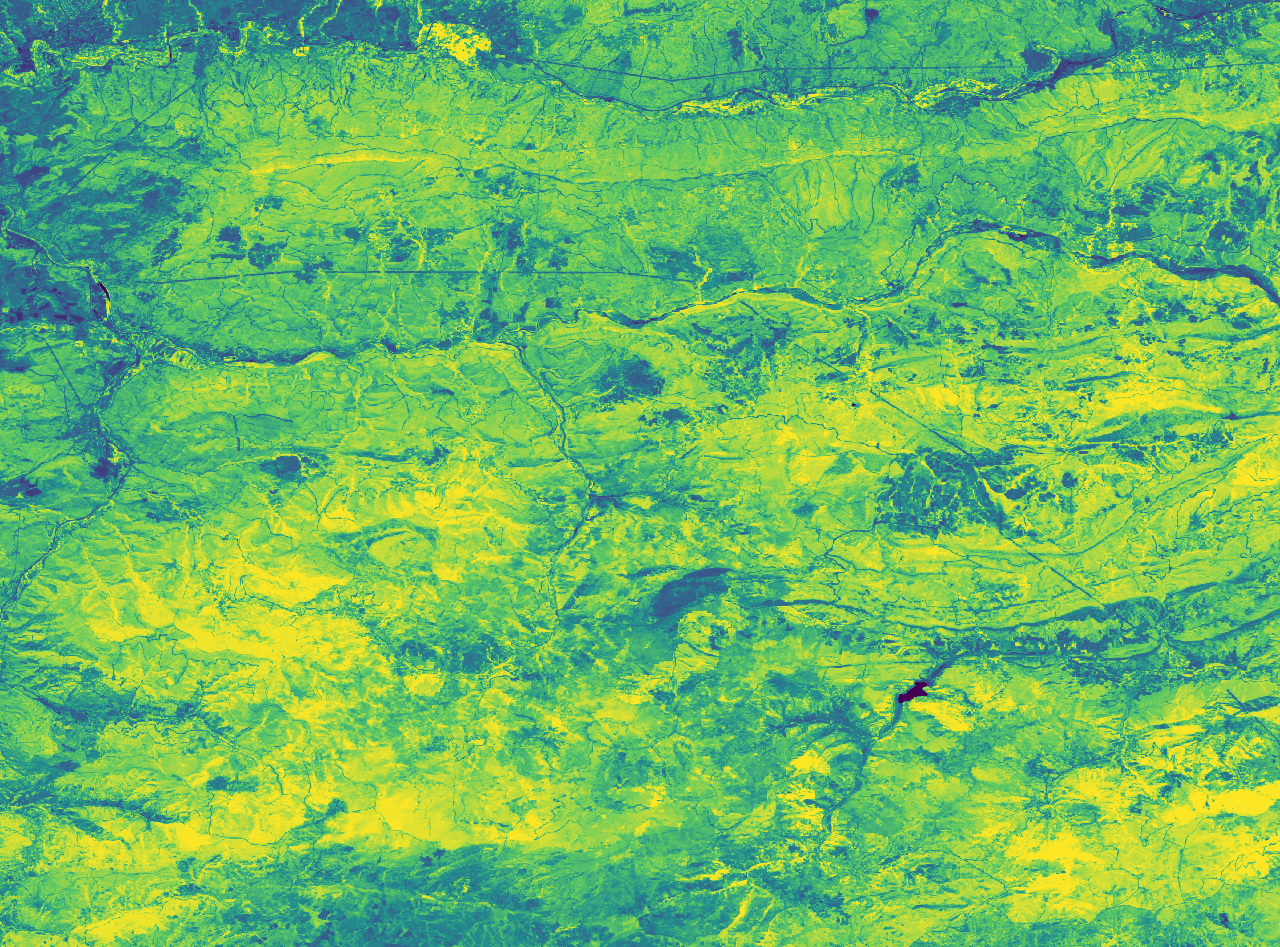
\includegraphics{../results/pre_NDVI.png}}
    \caption{Öncesi NDVI}
  \end{subfigure}\hfill
  \begin{subfigure}[b]{0.48\textwidth}
    \centering
    \resizebox{\linewidth}{!}{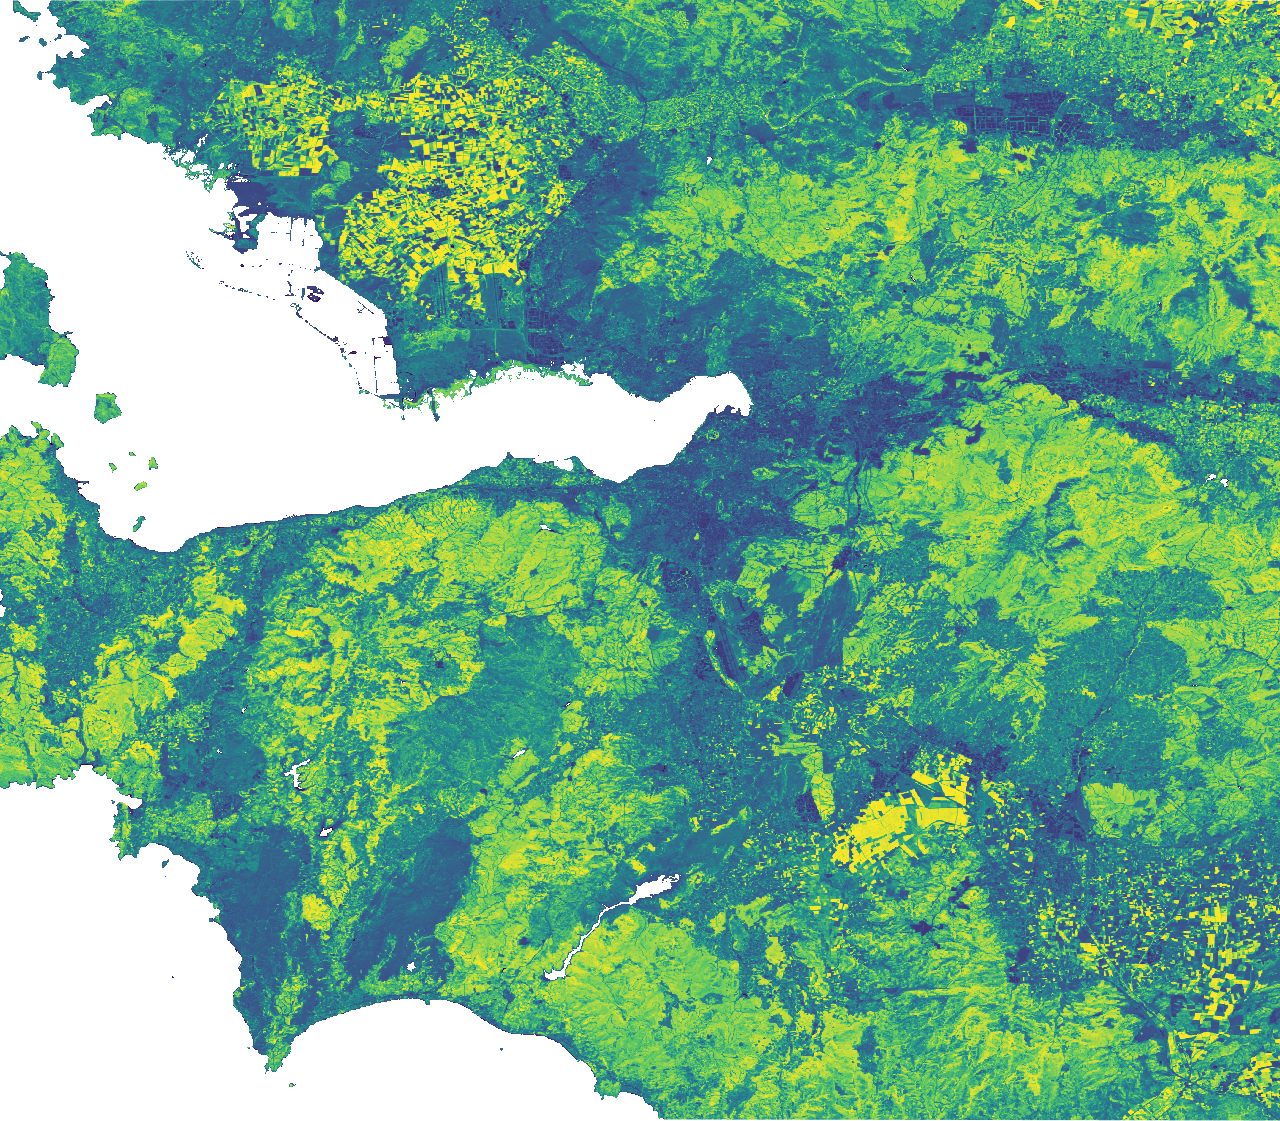
\includegraphics{../results/post_NDVI.png}}
    \caption{Sonrası NDVI}
  \end{subfigure}
  \caption{NDVI karşılaştırması.}
  \label{fig:ndvi}
\end{figure}

\begin{figure}[h]
  \centering
  \begin{subfigure}[b]{0.48\textwidth}
    \centering
    \resizebox{\linewidth}{!}{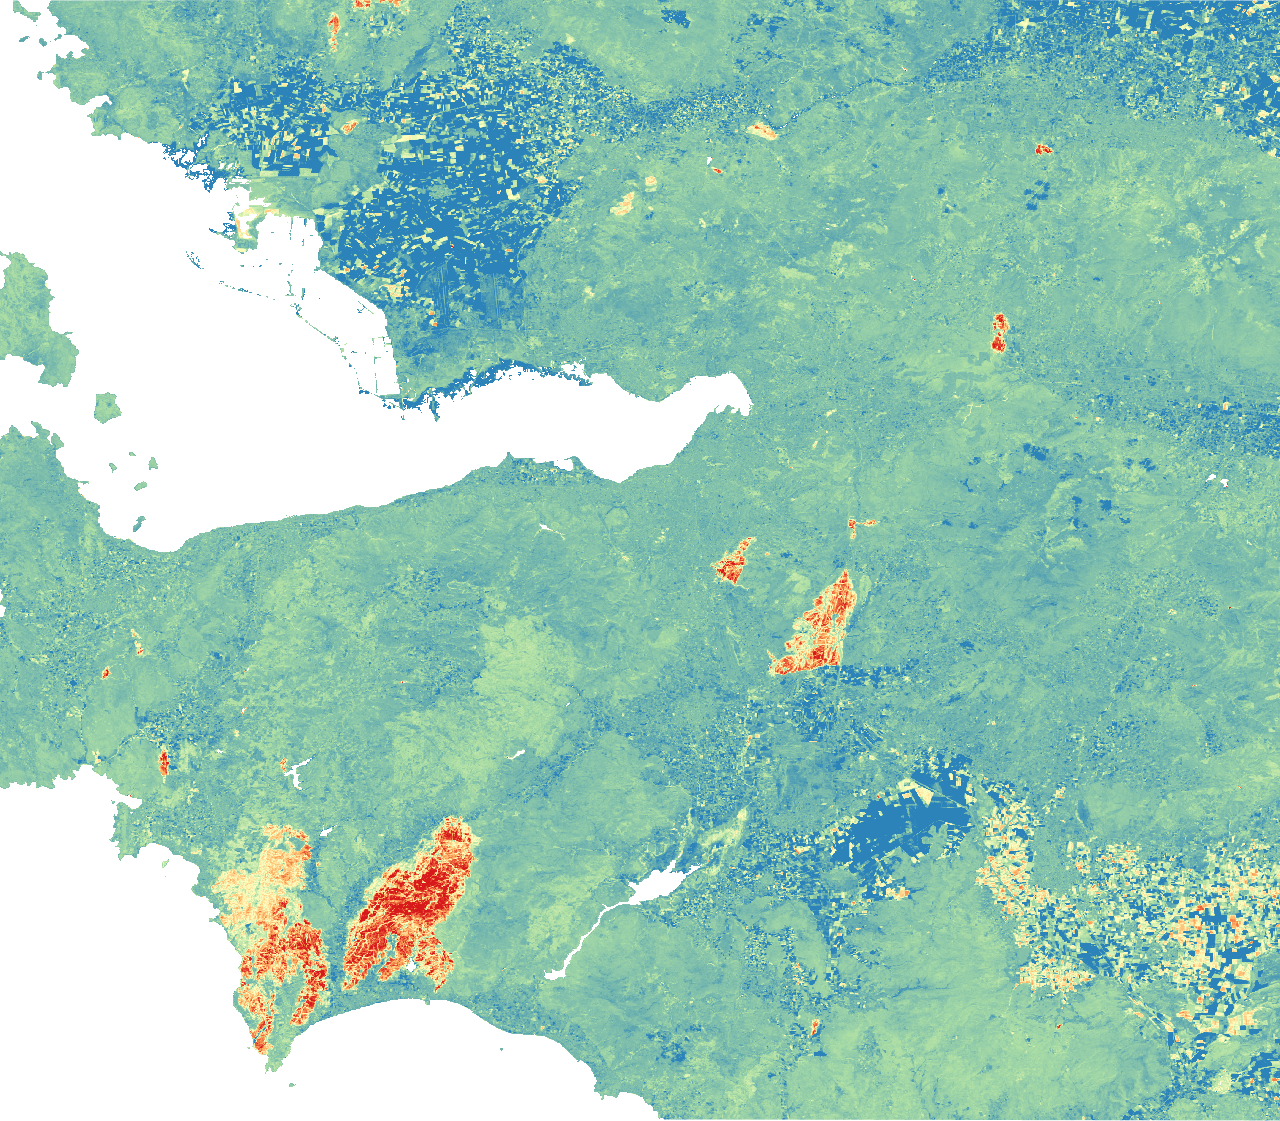
\includegraphics{../results/dNBR.png}}
    \caption{dNBR}
  \end{subfigure}\hfill
  \begin{subfigure}[b]{0.48\textwidth}
    \centering
    \resizebox{\linewidth}{!}{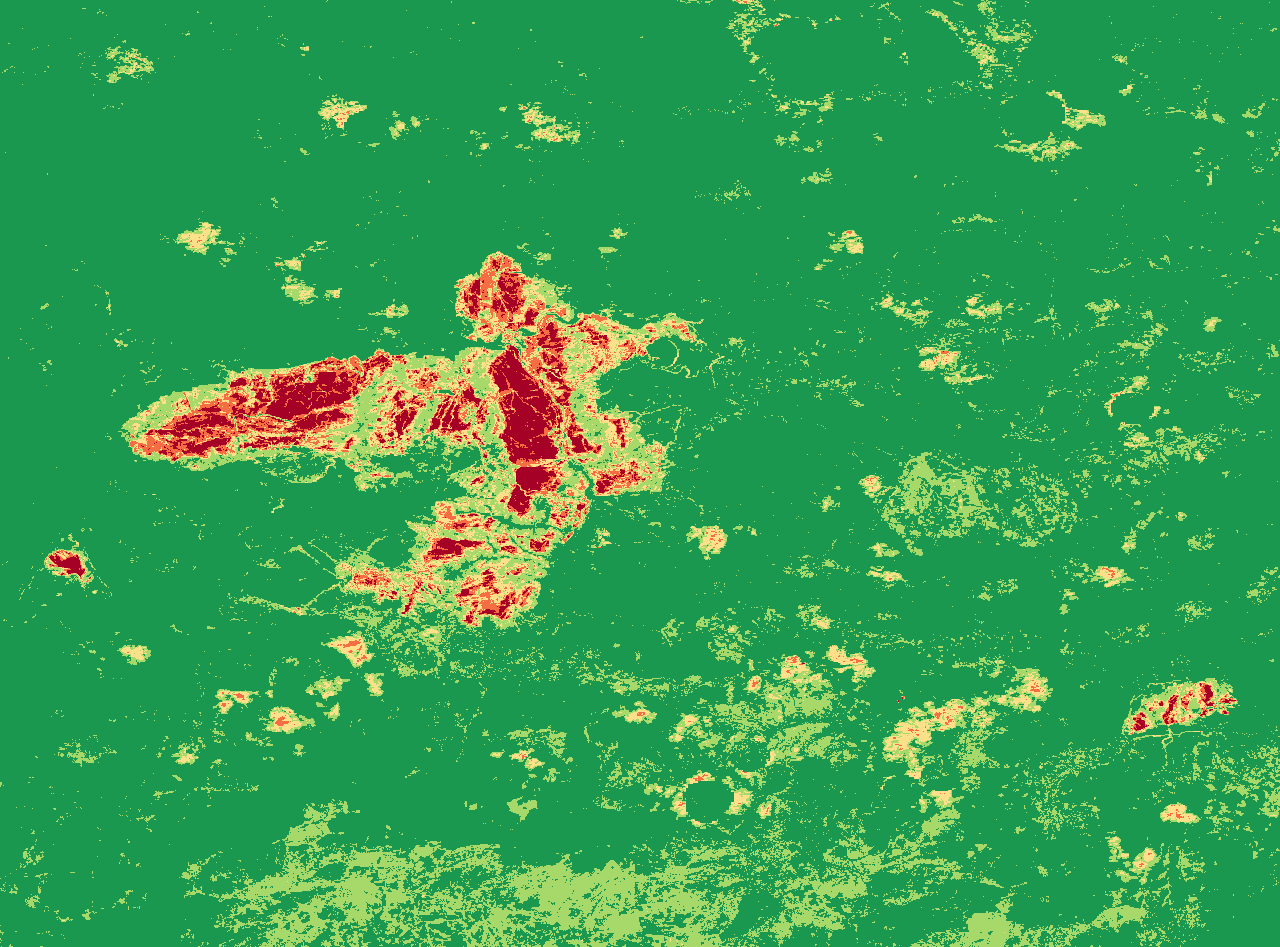
\includegraphics{../results/severity.png}}
    \caption{dNBR Şiddeti (0--4)}
  \end{subfigure}
  \caption{Fark analizi ve şiddet sınıfları.}
  \label{fig:diffs}
\end{figure}

\subsection*{Özet İstatistikler}
\begin{table}[h]
  \centering
  \begin{tabular}{@{}ll@{}}\toprule
  Metrik & Değer \\\midrule
  Öncesi Ortalama NDVI & 0.54 \\
  Sonrası Ortalama NDVI & 0.47 \\
  Ortalama dNDVI & $-0.06$ \\
  Ortalama dNBR & 0.07 \\\bottomrule
  \end{tabular}
  \caption{AOI genelinde özet istatistikler (örnek yer tutucu). Gerçek değerlere \texttt{../results/summary\_stats.csv} dosyasından erişilebilir.}
\end{table}

\paragraph{Yorum ve Anlamlandırma} Öncesi ve sonrası ortalama NDVI değerleri, AOI'deki
vejetasyonun yangın öncesi göreli canlılık düzeyi ile yangın sonrası durumunu özetler.
Bu iki değer arasındaki fark \(\Delta\mathrm{NDVI}\) (yaklaşık olarak \(\overline{\mathrm{dNDVI}}\)) negatif ise
genel vejetasyon kaybına işaret eder; büyüklüğü arttıkça kayıp şiddeti artar. Ortalama
\(\mathrm{dNDVI}\)'nin negatif olması, piksel ölçeğinde yaygın bir azalma sinyalinin
biriktiğini gösterir; ancak fenoloji (mevsimsellik), sulak alanlar veya tarımsal hasatlar
gibi faktörler yorumda dikkate alınmalıdır. Ortalama \(\mathrm{dNBR}\)'nin pozitif olması,
yanıklık göstergesi olan NBR düşüşünün AOI genelinde baskın olduğunu gösterir. \(\mathrm{dNBR}\)
değerinin kendisi doğrudan alanı değil, spektral değişim büyüklüğünü temsil eder; alan
 hesapları için sınıf piksel sayıları üzerinden türetim yapılmalıdır.

Bu çalışmada hesaplanan ortalamalar: öncesi NDVI yaklaşık 0.54, sonrası NDVI yaklaşık 0.47, dNDVI yaklaşık -0.06 ve dNBR yaklaşık 0.07'dir. Bu değerler, AOI genelinde çoğunlukla çok düşük/düşük yangın şiddetine işaret etmektedir.

\begin{table}[h]
  \centering
  \begin{tabular}{@{}llll@{}}\toprule
  Sınıf & Kod & Alan (ha) & Piksel Sayısı \\\midrule
  Yanıksız/Düşük & 0 & -- & -- \\
  Düşük & 1 & -- & -- \\
  Orta--Düşük & 2 & -- & -- \\
  Orta--Yüksek & 3 & -- & -- \\
  Yüksek & 4 & -- & -- \\\bottomrule
  \end{tabular}
  \caption{dNBR şiddet sınıfları için alan ve piksel sayıları (yer tutucu). Gerçek değerler sınıf piksel sayılarının piksel alanı ile çarpılmasıyla elde edilir.}
\end{table}

Etkilenen alan büyüklükleri, sınıf piksel sayıları ve/veya eşiklerin literatürle
karşılaştırılması ek bir tablo olarak verilebilir. RGB karşılaştırmaları (\ref{fig:rgb})
ve NDVI çiftleri (\ref{fig:ndvi}) mekânsal örüntülerin görsel olarak doğrulanmasına
yardımcı olurken, dNBR ve şiddet haritaları (\ref{fig:diffs}) farkların büyüklüğü ve
olası hasar zonlarının ayrımını destekler.

\section{Sınırlılıklar ve Belirsizlikler}
Bulut ve duman kalıntıları, geometrik/atmosferik kalıntı hataları ve sınıflandırma
eşiklerinin genellenebilirliği sonuçları etkileyebilir. dNBR eşikleri AOI'ye ve saha
gözlemlerine göre kalibre edilmelidir. Kompozit stratejisinin (median) seçimi mekânsal
özgüllük ve bulutluluk koşullarına bağlıdır.

\section{Tartışma ve Gelecek Çalışmalar}
Yöntem, GEE altyapısıyla hızlı ve tekrarlanabilir analiz sağlar. Gelecekte RdNBR gibi
normalize edilmiş fark metriklerinin denenmesi; arazi örtüsü/sınıf bilgisi ile
birleştirilmiş analizler ve saha verisiyle karşılaştırmalı doğrulama, karar destek
perspektifinden yöntemin değerini artıracaktır. Ayrıca farklı sensörlerle (Landsat,\,Sentinel-1)
çoklu-kaynak yaklaşımı geliştirilerek zamansal kapsam ve sağlamlık genişletilebilir.

\section{Görselleştirme}
Harita görselleri, \texttt{analysis.ipynb} defterinden otomatik üretilen HTML ve PNG
çıktıları üzerinden alınmıştır. Renk paletleri ve gösterim aralıkları \texttt{src/visualize.py}
dosyasında \texttt{vis\_params()} fonksiyonunda tanımlıdır.

\section{Veri ve Kod Erişimi}
Analiz akışı ve üretimler depo kökünde yer alan \texttt{analysis.ipynb} defteri ve
\texttt{src/} altındaki Python modülleri üzerinden yinelenebilir. Harita ve rapor
görselleri \texttt{results/} dizininde üretilmektedir. AOI tanımı \texttt{src/aoi.geojson}
dosyasında sağlanmıştır.

\section{Sonuç ve Tartışma}
Sunulan yöntem, GEE üzerinde hızlı ve tekrarlanabilir bir akışla yangın etkilerini
haritalandırmaktadır. Eşiklerin saha verileri ile kalibre edilmesi ve farklı
zaman aralıklarının denenmesiyle, hem doğruluk hem de yorumlanabilirlik artacaktır.
Gelecek çalışmalarda, \emph{Relative dNBR (RdNBR)} ve arazi örtüsü sınıflarıyla
birleşik değerlendirmeler önerilir.

\begin{thebibliography}{9}
\bibitem{Rouse1973} Rouse, J.W., Haas, R.H., Schell, J.A., Deering, D.W. (1973). Monitoring vegetation systems in the Great Plains with ERTS. In: Third ERTS Symposium.
\bibitem{KeyBenson2006} Key, C.H., Benson, N.C. (2006). Landscape Assessment: Ground measure of severity, the Composite Burn Index; and remote sensing of severity, the Normalized Burn Ratio. In: FIREMON.
\bibitem{Drusch2012} Drusch, M., et al. (2012). Sentinel-2: ESA's optical high-resolution mission for GMES operational services. Remote Sensing of Environment, 120, 25–36.
\end{thebibliography}

\end{document}
